\chapter{Cadre Général du Projet}

\section{Présentation de l'organisme d'accueil}

\subsection{Tunisie Telecom}

\TT{}, fondée en 1995 et privatisée partiellement en 2006, est l'opérateur historique de télécommunications en Tunisie. Avec plus de 7~millions d'abonnés fixes et mobiles, elle fournit des services de téléphonie, d'accès Internet haut débit (ADSL, fibre optique) et de solutions entreprise.

\TT{} dispose d'une infrastructure réseau couvrant l'ensemble du territoire tunisien, incluant :
\begin{itemize}
  \item Un réseau cœur IP/MPLS interconnectant les différentes régions.
  \item Des data centers hébergeant les services cloud et d'hébergement.
  \item Une plate-forme IoT en cours de déploiement pour les projets Smart City et industrie~4.0.
\end{itemize}

\subsection{Contexte du stage}

Le stage s'est déroulé au sein de l'équipe \textbf{Sécurité des Réseaux} de \TT{}, sous la supervision de \textbf{M. Moez KHLIFI}. L'équipe est en charge de la surveillance, de l'audit et du durcissement des infrastructures télécom de l'opérateur. Le projet PFE s'inscrit dans la stratégie de \TT{} visant à évaluer les solutions de sécurité adaptées aux déploiements IoT à grande échelle.

\subsection{Sujet du projet}

Le sujet confié porte sur la \textbf{sécurisation des flux de communication pour un écosystème IoT simulé}. Il s'agit de concevoir, déployer et valider une architecture de sécurité de bout en bout (E2E) couvrant :
\begin{itemize}
  \item L'authentification des dispositifs via une PKI dynamique.
  \item Le chiffrement des communications MQTT par TLS~1.3 avec authentification mutuelle (mTLS).
  \item La détection d'intrusions réseau par un IDS (Suricata).
  \item L'agrégation et la corrélation des événements de sécurité par un SIEM (Wazuh).
  \item La détection d'anomalies comportementales par des algorithmes de Machine Learning.
\end{itemize}

\section{Méthodologie de travail : Scrum}

\subsection{Choix de la méthodologie}

Pour mener à bien ce projet, nous avons adopté la méthodologie \textbf{Scrum}, un cadre de travail agile itératif et incrémental. Ce choix est motivé par :
\begin{itemize}
  \item La nature exploratoire du projet, nécessitant des ajustements fréquents de l'architecture.
  \item La nécessité de livrer des incréments fonctionnels à chaque itération pour validation par l'encadrant.
  \item La durée limitée du stage (environ 4 mois), imposant une gestion rigoureuse du temps et des priorités.
\end{itemize}

\subsection{Principes Scrum appliqués}

Scrum repose sur trois piliers fondamentaux : la \textbf{transparence}, l'\textbf{inspection} et l'\textbf{adaptation}. Dans le cadre de ce PFE, ces principes se sont traduits par :

\begin{description}
  \item[Transparence] Un journal de bord (\texttt{JOURNAL.md}) consigne quotidiennement les avancées, les blocages et les décisions techniques. L'intégralité du code source est versionné sous Git.
  \item[Inspection] Des points d'avancement hebdomadaires avec l'encadrante universitaire (Mme.~ELLOUZE) et des revues bimensuelles avec l'encadrant entreprise (M.~KHLIFI) permettent de valider les livrables.
  \item[Adaptation] Le Product Backlog est réajusté à chaque fin de sprint en fonction des résultats obtenus et des nouvelles contraintes identifiées.
\end{description}

\subsection{Rôles Scrum}

\begin{table}[H]
\centering
\caption{Répartition des rôles Scrum dans le projet}
\label{tab:roles_scrum}
\begin{tabular}{llp{6.5cm}}
\toprule
\textbf{Rôle} & \textbf{Personne} & \textbf{Responsabilité} \\
\midrule
Product Owner & M. Moez KHLIFI & Définition des besoins métier, priorisation du backlog, validation des livrables \\
Scrum Master & Mme. ELLOUZE NOURHENE & Suivi de l'avancement, levée des blocages, revue académique \\
Équipe de développement & Amine GHANNOUCHI & Conception, implémentation, tests, documentation \\
\bottomrule
\end{tabular}
\end{table}

\subsection{Artefacts Scrum}

\begin{description}
  \item[Product Backlog] Liste priorisée de toutes les fonctionnalités et tâches techniques du projet, découpée en \textit{user stories} et tâches techniques (voir tableau~\ref{tab:product_backlog}).
  \item[Sprint Backlog] Sous-ensemble du Product Backlog sélectionné pour chaque sprint, avec les critères d'acceptation associés.
  \item[Incrément] Livrable fonctionnel et testé produit à la fin de chaque sprint (composant déployé, tests validés, documentation associée).
\end{description}

\subsection{Cérémonies Scrum}

\begin{table}[H]
\centering
\caption{Cérémonies Scrum et leur application au projet}
\label{tab:ceremonies_scrum}
\begin{tabular}{lll}
\toprule
\textbf{Cérémonie} & \textbf{Fréquence} & \textbf{Participants} \\
\midrule
Sprint Planning & Début de sprint & PO, SM, Dev \\
Daily Stand-up & Quotidien (journal) & Dev (auto-suivi) \\
Sprint Review & Fin de sprint & PO, SM, Dev \\
Sprint Retrospective & Fin de sprint & SM, Dev \\
\bottomrule
\end{tabular}
\end{table}

\section{Product Backlog}

Le Product Backlog initial a été établi lors du Sprint~0 (cadrage) et affiné itérativement. Le tableau~\ref{tab:product_backlog} présente les principales \textit{user stories} et tâches techniques.

\begin{longtable}{clp{7.5cm}c}
\caption{Product Backlog du projet}\label{tab:product_backlog}\\
\toprule
\textbf{ID} & \textbf{Priorité} & \textbf{Description} & \textbf{Sprint} \\
\midrule
\endfirsthead
\toprule
\textbf{ID} & \textbf{Priorité} & \textbf{Description} & \textbf{Sprint} \\
\midrule
\endhead
US-01 & Haute & Installer et configurer GNS3 avec VMware & 1 \\
US-02 & Haute & Créer la topologie réseau avec VLANs & 1 \\
US-03 & Haute & Déployer pfSense et MikroTik CHR & 1 \\
US-04 & Haute & Valider la connectivité inter-VLAN & 1 \\
US-05 & Haute & Déployer Vault et activer le moteur PKI & 2 \\
US-06 & Haute & Créer la hiérarchie CA racine + intermédiaire & 2 \\
US-07 & Haute & Configurer Mosquitto en TLS~1.3/mTLS & 2 \\
US-08 & Haute & Automatiser l'émission des certificats & 2 \\
US-09 & Moyenne & Développer le simulateur de flotte IoT & 3 \\
US-10 & Moyenne & Injecter le dataset CSV (76\,000 événements) & 3 \\
US-11 & Moyenne & Déployer Suricata avec règles MQTT & 4 \\
US-12 & Moyenne & Déployer Wazuh OVA et configurer l'ingestion & 4 \\
US-13 & Moyenne & Développer le pipeline ML (IF + RF) & 4 \\
US-14 & Basse & Réaliser les tests de performance TLS & 4 \\
US-15 & Basse & Rédiger le rapport et préparer la soutenance & 5 \\
\bottomrule
\end{longtable}

\section{Planification des sprints}

Le projet est organisé en \textbf{six sprints} d'une durée de deux à trois semaines chacun, comme illustré par la figure~\ref{fig:scrum_sprints}.

\begin{figure}[H]
  \centering
  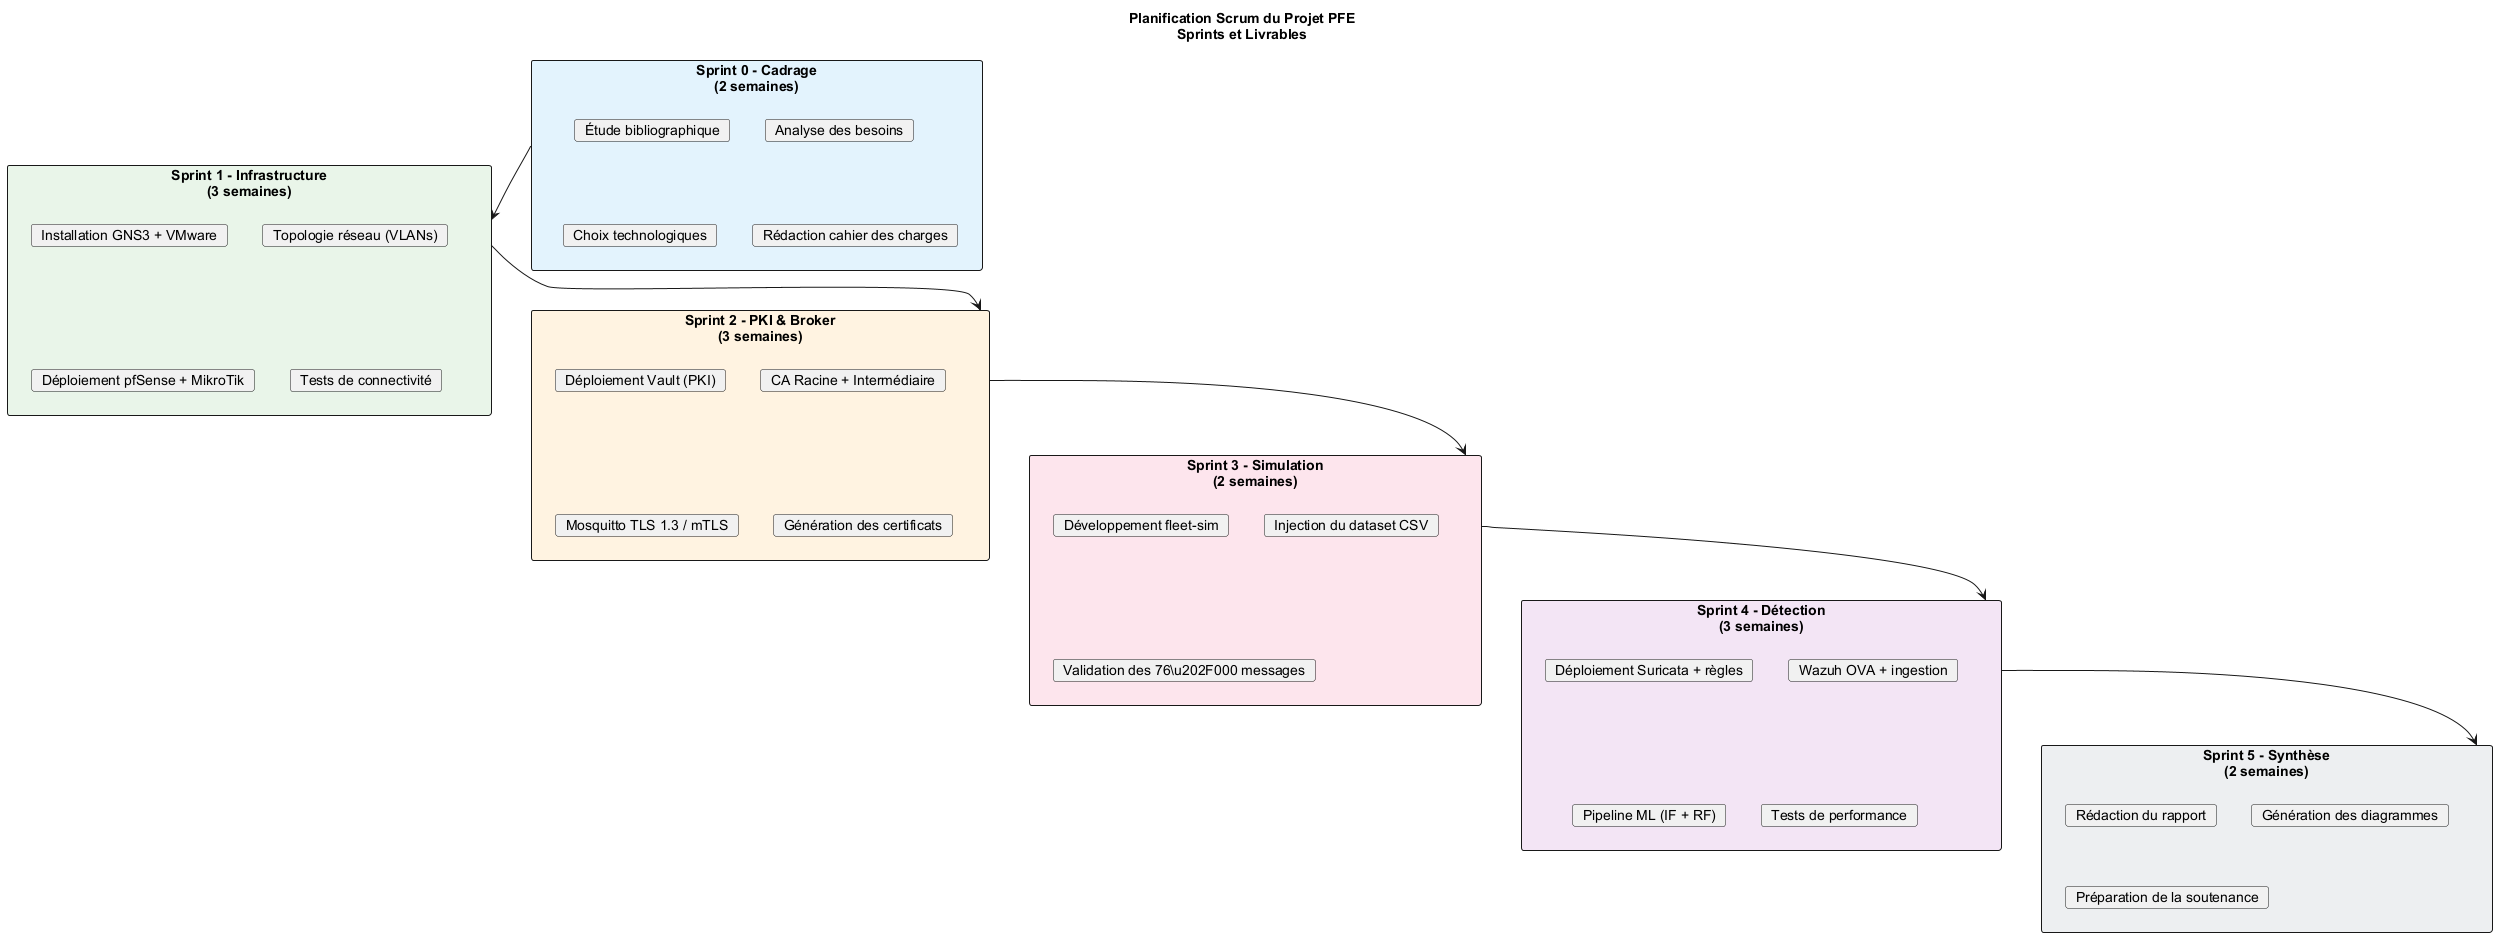
\includegraphics[width=\textwidth]{diagrams/diag-scrum-sprints.png}
  \caption{Planification des sprints du projet PFE}
  \label{fig:scrum_sprints}
\end{figure}

\subsection{Sprint 0 -- Cadrage (2 semaines)}

\begin{itemize}
  \item Analyse des besoins fonctionnels et non fonctionnels.
  \item Étude bibliographique : protocoles IoT, TLS/mTLS, PKI, SIEM, ML.
  \item Choix des technologies et outils (GNS3, Vault, Mosquitto, Suricata, Wazuh, scikit-learn).
  \item Rédaction du cahier des charges et validation par le Product Owner.
\end{itemize}

\textbf{Livrable :} Cahier des charges validé, architecture cible définie.

\subsection{Sprint 1 -- Infrastructure réseau (3 semaines)}

\begin{itemize}
  \item Installation de GNS3 et VMware Workstation Pro sur la machine hôte.
  \item Création de la topologie réseau avec trois VLANs (IoT, Services, Management).
  \item Déploiement de pfSense CE comme pare-feu périphérique.
  \item Configuration de MikroTik CHR pour le routage inter-VLAN.
  \item Tests de connectivité et validation des règles de firewall.
\end{itemize}

\textbf{Livrable :} Topologie réseau opérationnelle dans GNS3, tests de connectivité validés.

\subsection{Sprint 2 -- PKI et broker MQTT (3 semaines)}

\begin{itemize}
  \item Déploiement de HashiCorp Vault en conteneur Docker.
  \item Création de la CA racine et de la CA intermédiaire.
  \item Définition des rôles d'émission (services et dispositifs IoT).
  \item Configuration du broker Mosquitto en TLS~1.3 strict avec mTLS obligatoire.
  \item Automatisation de l'émission des 50 certificats de dispositifs.
  \item Validation de la chaîne de confiance complète.
\end{itemize}

\textbf{Livrable :} PKI fonctionnelle, broker MQTT sécurisé, 50 certificats émis.

\subsection{Sprint 3 -- Simulation de la flotte (2 semaines)}

\begin{itemize}
  \item Développement du simulateur de flotte IoT en Python (multi-thread).
  \item Chargement et partitionnement du dataset CSV entre 50 dispositifs simulés.
  \item Injection des 76\,000 messages MQTT en mTLS.
  \item Validation de la capture réseau par Suricata.
\end{itemize}

\textbf{Livrable :} 76\,000 messages publiés en mTLS, capture réseau disponible.

\subsection{Sprint 4 -- Détection et analyse (3 semaines)}

\begin{itemize}
  \item Déploiement de Suricata v7.0 avec le décodeur MQTT natif.
  \item Rédaction de quatre règles IDS personnalisées (DoS, injection, scanning, MiTM).
  \item Déploiement de Wazuh v4.7 (OVA) et configuration de l'ingestion des alertes Suricata.
  \item Création des règles de corrélation Wazuh personnalisées.
  \item Développement du pipeline ML : IsolationForest + RandomForest.
  \item Exécution des tests de performance (latence, RTT, débit).
\end{itemize}

\textbf{Livrable :} 51 alertes Suricata, dashboard Wazuh, modèles ML entraînés (F1 RF = 0,994).

\subsection{Sprint 5 -- Synthèse et documentation (2 semaines)}

\begin{itemize}
  \item Rédaction du rapport de PFE.
  \item Génération des diagrammes UML (PlantUML).
  \item Préparation de la présentation de soutenance.
  \item Revue finale avec les encadrants.
\end{itemize}

\textbf{Livrable :} Rapport final, support de soutenance.

\section{Diagramme de cas d'utilisation général}

La figure~\ref{fig:cas_utilisation} présente le diagramme de cas d'utilisation global du système, identifiant les trois acteurs principaux et leurs interactions.

\begin{figure}[H]
  \centering
  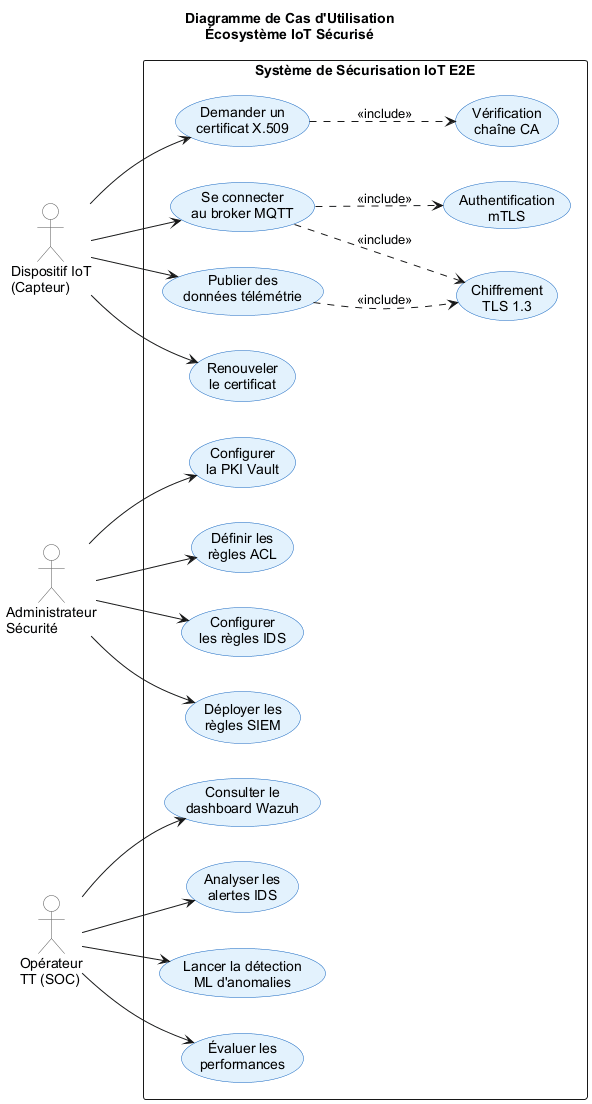
\includegraphics[width=0.85\textwidth]{diagrams/diag-cas-utilisation.png}
  \caption{Diagramme de cas d'utilisation du système IoT sécurisé}
  \label{fig:cas_utilisation}
\end{figure}

Les trois acteurs identifiés sont :
\begin{description}
  \item[Dispositif IoT] Demande un certificat, établit une connexion mTLS, publie des données de télémétrie.
  \item[Administrateur] Gère la PKI, configure les politiques de sécurité, surveille les performances.
  \item[Analyste SOC] Consulte les alertes Suricata/Wazuh, analyse les anomalies ML, gère les incidents.
\end{description}
